\section{Pure Computation}
\label{sec:timedriven_firststep}
As described in Chapter \ref{sec:back_frp}, Arrowized FRP \cite{hughes_generalising_2000} is a way to implement systems with continuous and discrete time semantics, where the central concept is the signal function, which can be understood as a process over time, mapping an input to an output signal. Early, non-arrowized implementations of FRP had the flaw that the $\Delta t$ or event $time$ itself was exposed, which could lead to non-causal signal functions. To make this more clear, we give an example of a signal function \texttt{futureSignal}, which returns a picture of a solid circle with radius 100, positioned at the coordinates of the mouse pointer \textit{100 years in the future}.

\begin{HaskellCode}
futureSignal :: Time -> Picture
futureSignal t = Translate p (circleSolid 100)
  where
    p = mousePosition (t + 100years)

mousePosition :: Time -> Position
\end{HaskellCode}

The problem is that the signal function \texttt{futureSignal}, does depend on a future mouse position, which directly leads to non-causality. Therefore it is not possible to run or simulate this program, at least not without inconsistencies.
Using Arrowized FRP with its implementation of signal functions as arrows, it is possible to solve this issue, as arrows parametrise also over the input type, thus making it possible to deal with this issue. Technically speaking, an arrowized signal function is a continuation which allows to capture state using closures and hides away the $\Delta t$. This has the result, that the $\Delta t$ can be hidden and therefore never be exposed explicitly to the programmer. Consequently the programmer can neither manipulate it nor define non-causal systems where a signal function depends on a signal in the future. We show more in technical detail how a signal function hides $\Delta t$ with the function \texttt{superSampling} in section \ref{sub:timedriven_results} below.

\medskip

As already pointed out, agents need to perceive time, which means that the concept of processes over time is an ideal match for agents and ABS as a whole, thus we will implement them and the whole system as signal functions.

According to the model, every agent makes \textit{on average} contact with $\beta$ random other agents per time unit. In ABS we can only contact discrete agents, thus we model this by generating a random event on average every $\frac{1}{\beta}$ time units. We need to sample from an exponential distribution because the rate is proportional to the size of the population \cite{borshchev_system_2004}. An agent does not know the other agents' states when making contact with them, thus we need a mechanism in which agents reveal the state in which they are in \textit{at the moment of making contact}. This mechanism is an implementation detail, which we will derive in our implementation steps. For now, we only assume that agents can contact each other somehow.

The \textit{parallel} strategy matches the semantics of the agent-based SIR model due to the underlying roots in the System Dynamics approach. As discussed already in Chapter \ref{sub:par_strategy}, in the parallel update strategy, the agents act conceptually all at the same time in lock-step. This implies that they observe the same system state during a time step and the actions of an agent are only visible in the next time step - they are isolated from each other. As will become apparent, functional programming can be used to enforce the correct application of this strategy, through the strong static type system, at compile time.

We start by defining the SIR states as Algebraic Data Type and our agents as signal functions (SF), which receive the SIR states of all agents form the previous step as input and outputs the current SIR state of the agent. This definition, and the fact that Yampa is not monadic, guarantees already at compile time, that the agents are isolated from each other, enforcing the \textit{parallel} lock-step semantics of the model.

\begin{HaskellCode}
data SIRState = Susceptible | Infected | Recovered

type SIRAgent = SF [SIRState] SIRState 

sirAgent :: RandomGen g => g -> SIRState -> SIRAgent
sirAgent g Susceptible = susceptibleAgent g
sirAgent g Infected    = infectedAgent g
sirAgent _ Recovered   = recoveredAgent
\end{HaskellCode}

Depending on the initial state, we return the corresponding behaviour. Also, we are passing a random number generator instead of running in the \texttt{Rand} Monad because signal functions as implemented in Yampa are not capable of being monadic. 

We see that the recovered agent ignores the random number generator because a recovered agent does nothing, stays immune forever and cannot get infected again in this model. Thus, a recovered agent is a consuming state from which there is no escape, it simply acts as a sink, constantly returning \texttt{Recovered}:

\begin{HaskellCode}
recoveredAgent :: SIRAgent
recoveredAgent = arr (const Recovered)
\end{HaskellCode}

Next, we implement the behaviour of a susceptible agent. It makes contact \textit{on average} with $\beta$ other random agents. For every \textit{infected} agent it contacts, it becomes infected with a probability of $\gamma$. If an infection happens, it makes the transition to the \texttt{Infected} state. To make contact, it gets fed the states of all agents in the system from the previous time step, so it can draw random contacts. Observing the states of all agents from the previous step allows for a very simple, one-directional form of making contact between agents. Although simple, it works perfectly for this approach in particular and for time-driven ABS in general. We will discuss a more complex interaction mechanism between agents in Chapter \ref{ch:eventdriven} on event-driven ABS.

A susceptible agent behaves as susceptible until it becomes infected. Upon infection an \texttt{Event} is returned, which results in switching into the \texttt{infectedAgent} SF, which causes the agent to behave as an infected agent from that moment on. When an infection event occurs, we change the behaviour of an agent using the Yampa combinator \texttt{switch}, which is quite elegant and expressive as it makes the change of behaviour at the occurrence of an event explicit. To make contact \textit{on average}, we use Yampas \texttt{occasionally} function which requires us to carefully select the right $\Delta t$ for sampling the system, as will be shown in the results below. 

The use of \texttt{iPre :: a $\rightarrow$ SF a a} delays the input signal by one sample, taking an initial value for the output at time zero. The reason for this is that we need to delay the transition from susceptible to infected by one step, due to the semantics of the \texttt{switch} combinator. Whenever the switching event occurs, the signal function into which is switched will be run at the time of the event occurrence. This means that a susceptible agent could make a transition to recovered within one time step. We want to prevent this occurrence, because the semantics should be that only one state transition can happen per time step.

\begin{HaskellCode}
susceptibleAgent :: RandomGen g => g -> SIRAgent
susceptibleAgent g 
    = switch 
      -- delay switching by 1 step to prevent against transition
      -- from Susceptible to Recovered within one time step
      (susceptible g >>> iPre (Susceptible, NoEvent)) 
      (const (infectedAgent g))
  where
    susceptible :: RandomGen g => g -> SF [SIRState] (SIRState, Event ())
    susceptible g = proc as -> do
      -- generate make contact events with given rate
      makeContact <- occasionally g (1 / beta) () -< ()
      if isEvent makeContact
        then (do
          -- draw random element from the list
          a <- drawRandomElemSF g -< as
          case a of
            Infected -> do
              -- returns True with uniform probability
              i <- randomBoolSF g gamma -< ()
              if i
                -- got infected, signal to switch through Event
                then returnA -< (Infected, Event ())
                else returnA -< (Susceptible, NoEvent)
             _       -> returnA -< (Susceptible, NoEvent))
        else returnA -< (Susceptible, NoEvent)
\end{HaskellCode}

To deal with randomness in an FRP way, we implemented additional signal functions built on the \texttt{noiseR} function provided by Yampa. This is an example of the stream character and statefulness of a signal function as it allows for keeping track of the changed random number generator internally, through the use of continuations and closures. Here we provide the implementation of \texttt{randomBoolSF}; \texttt{drawRandomElemSF} works similarly, but takes a list as input and returns a randomly chosen element from it:

\begin{HaskellCode}
randomBoolSF :: RandomGen g => g -> Double -> SF () Bool
randomBoolSF g p = proc _ -> do
  r <- noiseR ((0, 1) :: (Double, Double)) g -< ()
  returnA -< (r <= p)
\end{HaskellCode}

An infected agent recovers \textit{on average} after $\delta$ time units. This is implemented by drawing the duration from an exponential distribution \cite{borshchev_system_2004} with $\lambda = \frac{1}{\delta}$ and making the transition to the \texttt{Recovered} state after this duration. Thus, the infected agent behaves as infected until it recovers, after which it behaves as a recovered agent by switching into \texttt{recoveredAgent}. As in the case of the susceptible agent, we use the \texttt{occasionally} function to generate the event when the agent recovers.

\begin{HaskellCode}
infectedAgent :: RandomGen g => g -> SIRAgent
infectedAgent g 
    = switch 
      -- delay switching by 1 step 
      (infected >>> iPre (Infected, NoEvent))
      (const recoveredAgent)
  where
    infected :: SF [SIRState] (SIRState, Event ())
    infected = proc _ -> do
      recEvt <- occasionally g delta () -< ()
      let a = event Infected (const Recovered) recEvt
      returnA -< (a, recEvt)
\end{HaskellCode}

For running the simulation we use Yampas function \texttt{embed}:

\begin{HaskellCode}
runSimulation :: RandomGen g => g -> Time -> DTime -> [SIRState] -> [[SIRState]]
runSimulation g t dt as 
    = embed (stepSimulation sfs as) ((), dts)
  where
    steps     = floor (t / dt)
    dts       = replicate steps (dt, Nothing)
    n         = length as
    (rngs, _) = rngSplits g n [] -- unique rngs for each agent
    sfs       = zipWith sirAgent rngs as
\end{HaskellCode}

What we need to implement next is a closed feedback loop, which is at the heart of every ABS. The authors of \cite{courtney_yampa_2003, nilsson_functional_2002} discusses implementing this in Yampa. The function \texttt{stepSimulation} is an implementation of such a closed feedback loop. It takes the current signal functions and states of all agents, runs them all in parallel and returns this step's new agent states. The use of \texttt{notYet} is required to delay switching by one step to break a potentially infinite recursive switching. This is necessary because we are recursively switching back into the \texttt{stepSimulation}. This would then result in the immediate evaluation of the next step, overriding the output of the current step, recursively switching back into \texttt{stepSimulation} and so on. The combinator \texttt{notYet} breaks this up by delaying the switching event by one step.

\begin{HaskellCode}
stepSimulation :: [SIRAgent] -> [SIRState] -> SF () [SIRState]
stepSimulation sfs as =
    dpSwitch
      -- feeding the agent states to each SF
      (\_ sfs' -> (map (\sf -> (as, sf)) sfs'))
      -- the signal functions
      sfs
      -- switching event, delay by one step to prevent
      -- infinite recursion
      (switchingEvt >>> notYet)
      -- recursively switch back into stepSimulation         
      stepSimulation                            
  where
    switchingEvt :: SF ((), [SIRState]) (Event [SIRState])
    switchingEvt = arr (\ (_, newAs) -> Event newAs)
\end{HaskellCode}

Yampa provides the \texttt{dpSwitch} combinator for running signal functions in parallel, which has the following type signature:

\begin{HaskellCode}
dpSwitch :: Functor col
         -- routing function
         => (forall sf. a -> col sf -> col (b, sf))
         -- SF collection
         -> col (SF b c)
         -- SF generating switching event     
         -> SF (a, col c) (Event d)
         -- continuation to invoke upon event           
         -> (col (SF b c) -> d -> SF a (col c))
         -> SF a (col c)
\end{HaskellCode}

Conceptually, \texttt{dpSwitch} allows us to recursively switch back into the \\ \texttt{stepSimulation} with the continuations and new states of all the agents after they were run in parallel. 

Its first argument is the pairing-function, which pairs up the input to the signal functions - it has to preserve the structure of the signal function collection. The second argument is the collection of signal functions to run. The third argument is a signal function generating the switching event. The last argument is a function, which generates the continuation after the switching event has occurred. \texttt{dpSwitch} returns a new signal function, which runs all the signal functions in parallel and switches into the continuation when the switching event occurs. %The d in \textit{dpSwitch} stands for delayed observation.

\subsection{Results}
\label{sub:timedriven_results}

The dynamics generated by this implementation can be seen in Figure \ref{fig:sir_abs_dynamics_frp}. 

\begin{figure}
\begin{center}
	\begin{tabular}{c c}
		\begin{subfigure}[b]{0.4\textwidth}
			\centering
			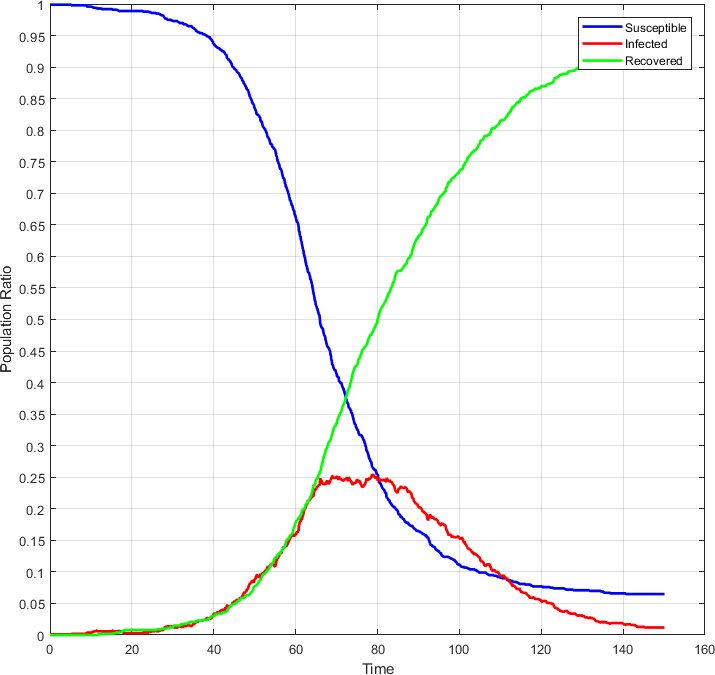
\includegraphics[width=1\textwidth, angle=0]{./fig/timedriven/SIR_Yampa/SIR_Yampa_dt01.png}
			\caption{$\Delta t = 0.1$}
			\label{fig:sir_abs_approximating_01dt_1000agents}
		\end{subfigure}
		
		&
    	
		\begin{subfigure}[b]{0.4\textwidth}
			\centering
			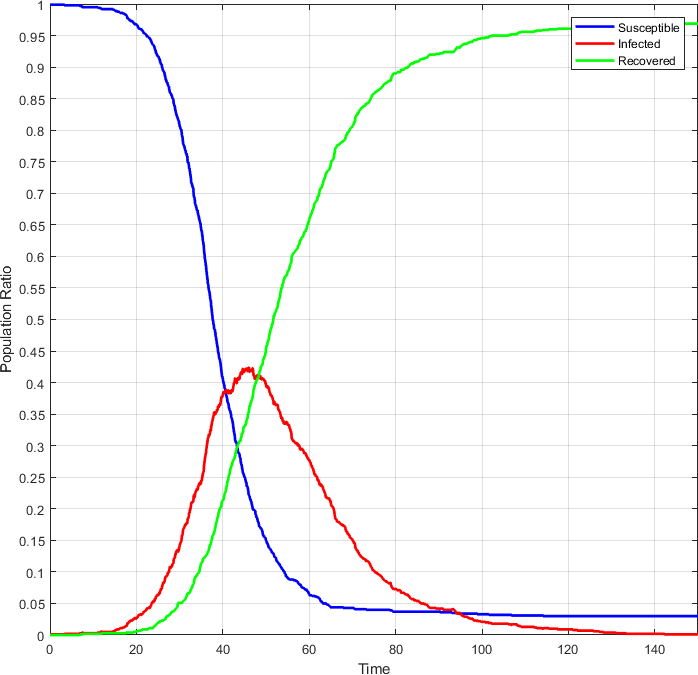
\includegraphics[width=1\textwidth, angle=0]{./fig/timedriven/SIR_Yampa/SIR_Yampa_dt001.png}
			\caption{$\Delta t = 0.01$}
			\label{fig:sir_abs_approximating_001dt_1000agents}
		\end{subfigure}
	\end{tabular}
	
	\caption[FRP simulation of agent-based SIR showing the influence of different $\Delta t$]{FRP simulation of agent-based SIR showing the influence of different $\Delta t$. Population size of 1,000 with contact rate $\beta = \frac{1}{5}$, infection probability $\gamma = 0.05$, illness duration $\delta = 15$ with initially 1 infected agent. Simulation run for 150 time steps with respective $\Delta t$.} 
	\label{fig:sir_abs_dynamics_frp}
\end{center}
\end{figure}

By following the FRP approach we assume a continuous flow of time, which means that we need to select a \textit{correct} $\Delta t$, otherwise we would end up with wrong dynamics. The selection of a correct $\Delta t$ depends, in our case, on \texttt{occasionally} in the susceptible behaviour, which randomly generates an event on average with $\beta$ following the exponential distribution. To arrive at the correct dynamics, this requires us to sample \texttt{occasionally}, and thus the whole system, with small enough $\Delta t$ matching the frequency of events generated by $\beta$. If we choose too large a $\Delta t$, we lose events, which will result in wrong dynamics as can be seen in Figure \ref{fig:sir_abs_approximating_01dt_1000agents}. This issue is known as undersampling and is described in Figure \ref{fig:sampling_issue}.

\begin{figure}
\begin{center}
	\begin{tabular}{c}
		\begin{subfigure}[b]{0.5\textwidth}
			\centering
			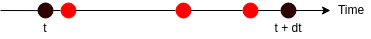
\includegraphics[width=1\textwidth, angle=0]{./fig/timedriven/undersampling.png}
			\caption{Under-sampling}
			\label{fig:undersampling}
		\end{subfigure}
		
		\\
		
		\begin{subfigure}[b]{0.5\textwidth}
			\centering
			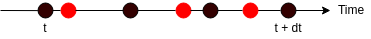
\includegraphics[width=1\textwidth, angle=0]{./fig/timedriven/supersampling.png}
			\caption{Super-sampling}
			\label{fig:supersampling}
		\end{subfigure}
	\end{tabular}
	
	\caption[Visual explanation of undersampling and supersampling]{Visual explanation of undersampling and supersampling. The black dots represent the time steps of the simulation. The red dots represent virtual events, which occur at specific points in continuous time. In the case of undersampling, three events occur in between the two time steps but \texttt{occasionally} only captures the first one. By increasing the sampling frequency either through a smaller $\Delta t$, or supersampling all three events can be captured.} 
	\label{fig:sampling_issue}
\end{center}
\end{figure}

For tackling this issue we have three options. The first one is to use a smaller $\Delta t$ as can be seen in \ref{fig:sir_abs_approximating_001dt_1000agents}, which results in the whole system being sampled more often, thus reducing performance. The second option is to step the simulation with $\Delta t = 1$ and in each step, instead of using \texttt{occasionally}, to make a number of contacts drawn from the exponential distribution. If we follow this option, we abandon the time-driven approach altogether because we don't abstract away from $\Delta t$. This option violates the fundamental abstraction of FRP, which assumes that time is continuous and signal functions are running conceptually infinitely fast and infinitely often \cite{winograd-cort_wormholes:_2012}. This leaves us with the third option to implement supersampling and apply it to \texttt{occasionally}, which allows us to run the whole simulation with $\Delta t = 1.0$ and only sample the \texttt{occasionally} function with a much higher frequency.

The function \texttt{embed}, which allows us to run a given signal function with provided $\Delta t$, does not help here because it does not return a signal function. What we need is a signal function which takes the number of super samples \texttt{n}, the signal function \texttt{sf} to sample and return a new signal function, which performs supersampling on it. We provide a full implementation of such a function. Additionally, this instance gives insight into how signal functions are implemented in Yampa, and how the $\Delta t$ is hidden:

\begin{HaskellCode}
-- SF is the signal function defined for time t = 0 and returns
-- a continuation of type SF' which is the signal function 
-- defined for t > 0: it receives an additional time delta
-- data SF a b  = SF { sfTF :: a -> (SF' a b, b) }
-- data SF' a b = DTime -> a -> (SF' a b, b)

superSampling :: Int -> SF a b -> SF a [b]
superSampling n sf0 = SF { sfTF = tf0 }
  where
    -- no supersampling at time 0
    tf0 :: a -> (SF' a b, [b])
    tf0 a0 = (tfCont, replicate n b0)
      where
        (sf', b0) = sfTF sf0 a0 -- running the SF using sfTF 
        tfCont    = superSamplingAux sf'

    superSamplingAux :: SF' a [b]
    superSamplingAux sf' = SF' tf
      where
        tf :: DTime -> a -> (SF' a b, [b])
        tf dt a = (tf', bs)
          where
            (sf'', bs) = superSampleRun n dt sf' a
            tf'        = superSamplingAux sf''

    superSampleRun :: Int -> DTime -> SF' a b -> a -> (SF' a b, [b])
    superSampleRun n dt sf a 
        | n <= 1    = superSampleMulti 1 dt sf a []
        | otherwise = (sf', reverse bs)  -- reverse due to accumulator
      where
        superDt   = dt / fromIntegral n
        (sf', bs) = superSampleMulti n superDt sf a []

    superSampleMulti :: Int -> DTime -> SF' a b -> a -> [b] -> (SF' a b, [b])
    superSampleMulti 0 _ sf _ acc  = (sf, acc)
    superSampleMulti n dt sf a acc = superSampleMulti (n-1) dt sf' a (b:acc) 
      where
        (sf', b) = sfTF' sf dt a -- running the SF' using sfTF'
\end{HaskellCode}

It evaluates the \texttt{SF} argument for \texttt{n} times, each with $\Delta t = \frac{\Delta t}{n}$ and the same input argument \texttt{a} for all \texttt{n} evaluations. At time 0 no super-sampling is performed and just a single output of the \texttt{SF} argument is calculated. A list of \texttt{b} is returned with length of \texttt{n} containing the result of the \texttt{n} evaluations of the \texttt{SF} argument. If 0 or less super samples are requested exactly one is calculated. %We could then wrap the occasionally function which would then generate a list of events. 

\subsection{Discussion}
We conclude that our first step already introduced most of the fundamental concepts of ABS:
\begin{itemize}
	\item Time - the simulation occurs over virtual time which is modelled explicitly, divided into \textit{fixed} $\Delta t$, where at each step all agents are executed.
	
	\item Agents - each agent is implemented as an individual, with the behaviour depending on its state. It is clear to see that agents behave as signals: when the system is sampled with $\Delta t = 0$ then their behaviour will stay constant and will not change because it is completely determined by the flow of time. 
	
	\item Feedback - the output state of the agent in the current time step $t$ is the input state for the next time step $t + \Delta t$.
	
	\item Environment - as environment we implicitly assume a fully connected network (complete graph) where every agent 'knows' every other agent, including itself and thus can make contact with all of them.
	
	\item Stochasticity - it is an inherently stochastic simulation, which is indicated by the random number generator and the usage of \texttt{occasionally}, \texttt{randomBoolSF} and \texttt{drawRandomElemSF}.
	
	\item Deterministic - repeated runs with the same initial randomnumber generator result in same dynamics. This may not come as a surprise, but in Haskell we can guarantee that property statically immediately at compile time because our simulation does \textit{not} run in the \texttt{IO} Monad. This guarantees that no external, uncontrollable sources of non-determinism can interfere with the simulation.
	
	\item Parallel, lock-step semantics - the simulation implements a \textit{parallel} update strategy, where in each step, the agents are run isolated in parallel and don't see the actions of the others until the next step.
\end{itemize}

Using FRP in Yampa results in a clear, expressive and robust implementation. State is implicitly encoded, depending on which signal function is active. By using explicit time semantics with \texttt{occasionally} we can achieve extremely fine grained stochastics by sampling the system with small $\Delta t$. We are treating it as a truly continuous time-driven agent-based system.

A severe problem, which is hard to find with testing, is the fact that in the susceptible agent the same random number generator is used in \texttt{occasionally}, \texttt{drawRandomElemSF} and \texttt{randomBoolSF}. This means that all three stochastic functions, which should be independent from each other, are inherently correlated. This is something one wants to prevent under all circumstances in a simulation, as it can invalidate the dynamics on a very subtle level. We left this severe bug in for explanatory reasons, as it shows an example where functional programming actually encourages very subtle bugs, if one is not careful. A possible, but not very elegant, solution would be to simply split the initial random number generator in \texttt{sirAgent} three times and pass three random number generators to \texttt{susceptibleAgent}. A much more elegant solution would be to use the \texttt{Rand} Monad, which unfortunately is not possible, because Yampa is not monadic.

So far we have an acceptable implementation of an agent-based SIR approach. What we are lacking at the moment is an elegant solution to the random number correlation and a general treatment of an environment. In the next step we make the transition to Monadic Stream Functions as introduced in Dunai \cite{perez_functional_2016}, which allows FRP within a monadic context and gives us a method for an elegant solution to the random number correlation.